\documentclass[14pt]{extbook}
\usepackage{multicol, enumerate, enumitem, hyperref, color, soul, setspace, parskip, fancyhdr} %General Packages
\usepackage{amssymb, amsthm, amsmath, bbm, latexsym, units, mathtools} %Math Packages
\everymath{\displaystyle} %All math in Display Style
% Packages with additional options
\usepackage[headsep=0.5cm,headheight=12pt, left=1 in,right= 1 in,top= 1 in,bottom= 1 in]{geometry}
\usepackage[usenames,dvipsnames]{xcolor}
\usepackage{dashrule}  % Package to use the command below to create lines between items
\newcommand{\litem}[1]{\item#1\hspace*{-1cm}\rule{\textwidth}{0.4pt}}
\pagestyle{fancy}
\lhead{Progress Quiz 5}
\chead{}
\rhead{Version B}
\lfoot{9912-2038}
\cfoot{}
\rfoot{Spring 2021}
\begin{document}

\begin{enumerate}
\litem{
Determine the vertical asymptotes and holes in the rational function below.\[ f(x) = \frac{8x^{3} +22 x^{2} -21 x -45}{8x^{2} -22 x + 15} \]\begin{enumerate}[label=\Alph*.]
\item \( \text{Vertical Asymptotes of } x = 1.25 \text{ and } x = -1.25 \text{ with a hole at } x = 1.5 \)
\item \( \text{Holes at } x = 1.25 \text{ and } x = 1.5 \text{ with no vertical asymptotes.} \)
\item \( \text{Vertical Asymptote of } x = 1.0 \text{ and hole at } x = 1.5 \)
\item \( \text{Vertical Asymptotes of } x = 1.25 \text{ and } x = 1.5 \text{ with no holes.} \)
\item \( \text{Vertical Asymptote of } x = 1.25 \text{ and hole at } x = 1.5 \)

\end{enumerate} }
\litem{
Determine the vertical asymptotes and holes in the rational function below.\[ f(x) = \frac{6x^{3} +43 x^{2} +91 x + 60}{4x^{2} +16 x + 15} \]\begin{enumerate}[label=\Alph*.]
\item \( \text{Vertical Asymptotes of } x = -2.5 \text{ and } x = -1.5 \text{ with no holes.} \)
\item \( \text{Holes at } x = -2.5 \text{ and } x = -1.5 \text{ with no vertical asymptotes.} \)
\item \( \text{Vertical Asymptote of } x = -2.5 \text{ and hole at } x = -1.5 \)
\item \( \text{Vertical Asymptotes of } x = -2.5 \text{ and } x = -1.667 \text{ with a hole at } x = -1.5 \)
\item \( \text{Vertical Asymptote of } x = 1.5 \text{ and hole at } x = -1.5 \)

\end{enumerate} }
\litem{
Determine the horizontal and/or oblique asymptotes in the rational function below.\[ f(x) = \frac{12x^{3} +32 x^{2} +x -30}{30x^{3} -68 x^{2} -71 x + 30} \]\begin{enumerate}[label=\Alph*.]
\item \( \text{Horizontal Asymptote of } y = 0.400  \)
\item \( \text{Vertical Asymptote of } y = -2  \)
\item \( \text{Vertical Asymptote of } y = 0.600  \)
\item \( \text{None of the above} \)
\item \( \text{Horizontal Asymptote of } y = 0  \)

\end{enumerate} }
\litem{
Determine the vertical asymptotes and holes in the rational function below.\[ f(x) = \frac{12x^{3} -29 x^{2} -33 x + 36}{9x^{2} -3 x -20} \]\begin{enumerate}[label=\Alph*.]
\item \( \text{Vertical Asymptote of } x = 1.333 \text{ and hole at } x = -1.333 \)
\item \( \text{Vertical Asymptotes of } x = 1.667 \text{ and } x = 0.75 \text{ with a hole at } x = -1.333 \)
\item \( \text{Holes at } x = 1.667 \text{ and } x = -1.333 \text{ with no vertical asymptotes.} \)
\item \( \text{Vertical Asymptotes of } x = 1.667 \text{ and } x = -1.333 \text{ with no holes.} \)
\item \( \text{Vertical Asymptote of } x = 1.667 \text{ and hole at } x = -1.333 \)

\end{enumerate} }
\litem{
Determine the vertical asymptotes and holes in the rational function below.\[ f(x) = \frac{12x^{3} + x^{2} -80 x + 75}{12x^{2} -5 x -25} \]\begin{enumerate}[label=\Alph*.]
\item \( \text{Holes at } x = -1.25 \text{ and } x = 1.667 \text{ with no vertical asymptotes.} \)
\item \( \text{Vertical Asymptote of } x = 1.0 \text{ and hole at } x = 1.667 \)
\item \( \text{Vertical Asymptotes of } x = -1.25 \text{ and } x = 1.25 \text{ with a hole at } x = 1.667 \)
\item \( \text{Vertical Asymptotes of } x = -1.25 \text{ and } x = 1.667 \text{ with no holes.} \)
\item \( \text{Vertical Asymptote of } x = -1.25 \text{ and hole at } x = 1.667 \)

\end{enumerate} }
\litem{
Which of the following functions \textit{could} be the graph below?
\begin{center}
    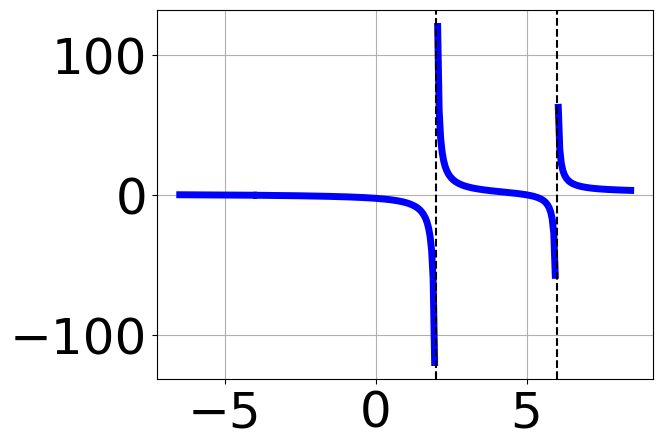
\includegraphics[width=0.5\textwidth]{../Figures/identifyGraphOfRationalFunctionCopyB.png}
\end{center}
\begin{enumerate}[label=\Alph*.]
\item \( f(x)=\frac{x^{3} -1 x^{2} -25 x + 25}{x^{3} +14 x^{2} +55 x + 42} \)
\item \( f(x)=\frac{x^{3} -31 x -30}{x^{3} -14 x^{2} +55 x -42} \)
\item \( f(x)=\frac{x^{3} -31 x + 30}{x^{3} +14 x^{2} +55 x + 42} \)
\item \( f(x)=\frac{x^{3} -31 x -30}{x^{3} -14 x^{2} +55 x -42} \)
\item \( \text{None of the above are possible equations for the graph.} \)

\end{enumerate} }
\litem{
Determine the horizontal and/or oblique asymptotes in the rational function below.\[ f(x) = \frac{9x^{3} +18 x^{2} -25 x -50}{3x^{2} -14 x + 15} \]\begin{enumerate}[label=\Alph*.]
\item \( \text{Horizontal Asymptote of } y = 3.0 \text{ and Oblique Asymptote of } y = 3x + 20 \)
\item \( \text{Horizontal Asymptote at } y = 3.0 \)
\item \( \text{Horizontal Asymptote of } y = 3.0 \text{ and Oblique Asymptote of } y = 3x + 20 \)
\item \( \text{Horizontal Asymptote of } y = 3.0  \)
\item \( \text{Oblique Asymptote of } y = 3x + 20. \)

\end{enumerate} }
\litem{
Determine the horizontal and/or oblique asymptotes in the rational function below.\[ f(x) = \frac{4x^{2} +19 x + 12}{16x^{3} +96 x^{2} +143 x + 60} \]\begin{enumerate}[label=\Alph*.]
\item \( \text{Horizontal Asymptote of } y = 0 \)
\item \( \text{Horizontal Asymptote at } y = -4.000 \)
\item \( \text{Oblique Asymptote of } y = 4x + 5. \)
\item \( \text{Horizontal Asymptote of } y = 0.250  \)
\item \( \text{Horizontal Asymptote of } y = 0.250 \text{ and Oblique Asymptote of } y = 4x + 5 \)

\end{enumerate} }
\litem{
Determine the horizontal and/or oblique asymptotes in the rational function below.\[ f(x) = \frac{12x^{3} +61 x^{2} +87 x + 36}{3x^{2} -5 x -12} \]\begin{enumerate}[label=\Alph*.]
\item \( \text{Horizontal Asymptote at } y = 3.0 \)
\item \( \text{Horizontal Asymptote of } y = 3.0 \text{ and Oblique Asymptote of } y = 4x + 27 \)
\item \( \text{Horizontal Asymptote of } y = 4.0 \text{ and Oblique Asymptote of } y = 4x + 27 \)
\item \( \text{Horizontal Asymptote of } y = 4.0  \)
\item \( \text{Oblique Asymptote of } y = 4x + 27. \)

\end{enumerate} }
\litem{
Which of the following functions \textit{could} be the graph below?
\begin{center}
    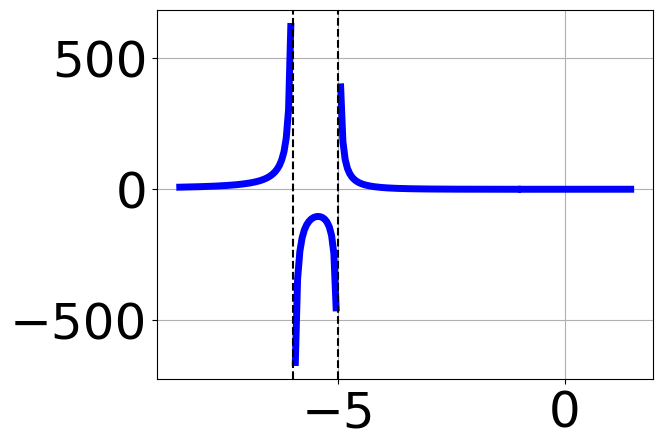
\includegraphics[width=0.5\textwidth]{../Figures/identifyGraphOfRationalFunctionB.png}
\end{center}
\begin{enumerate}[label=\Alph*.]
\item \( f(x)=\frac{x^{3} -12 x^{2} +47 x -60}{x^{3} +5 x^{2} -18 x -72} \)
\item \( f(x)=\frac{x^{3} +12 x^{2} +47 x + 60}{x^{3} -5 x^{2} -18 x + 72} \)
\item \( f(x)=\frac{x^{3} -13 x^{2} +55 x -75}{x^{3} +5 x^{2} -18 x -72} \)
\item \( f(x)=\frac{x^{3} +12 x^{2} +47 x + 60}{x^{3} -5 x^{2} -18 x + 72} \)
\item \( \text{None of the above are possible equations for the graph.} \)

\end{enumerate} }
\end{enumerate}

\end{document}